\documentclass{beamer}
\usepackage{graphicx}
\title{Das Ziegenspiel}
\subtitle{Unintuitive Wahrscheinlichkeiten}

%\usetheme{lucid}
\begin{document}
	\frame {
		\titlepage
	}
	\frame {
		\frametitle{Was ist das Ziegenspiel?}
		Bei dem Ziegenspiel gibt es drei Türen, hinter einer dieser Türen gibt es einen Preis, hinter den anderen beiden stehen Ziegen. Nachdem man eine Tür wählt, offenbart der Moderator, dass sich hinter einer der beiden ungeöffneten Türen eine Ziege verbirgt. Anschließend wird man gefragt, ob man wechseln möchte.
		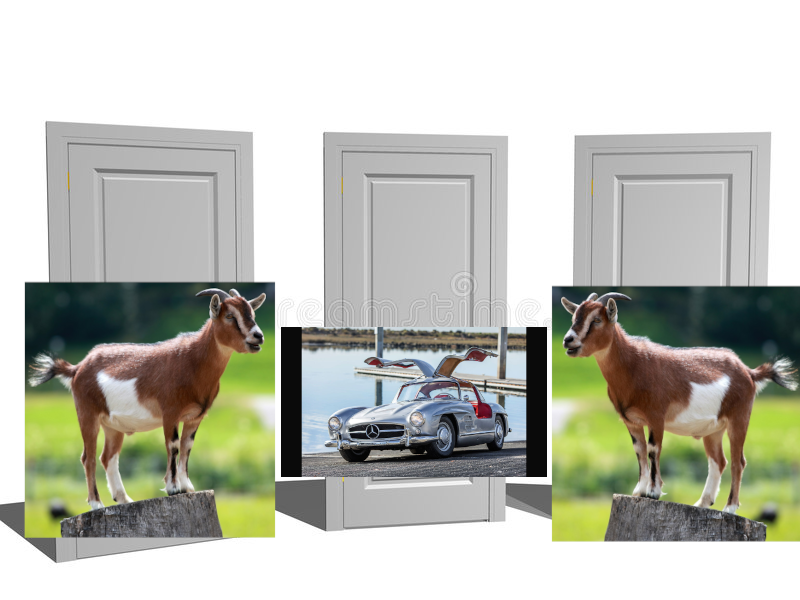
\includegraphics{dreitueren}
	}
	\frame{
		\frametitle{Die Optimale Strategie}
		\framesubtitle{Gibt es überhaupt eine optimale Strategie, was meint ihr?}
	}
	\frame{
		\frametitle{Simulation}
		Die Lösung: eine Simulation
	}
	\frame{
		\frametitle{Ausgedrückt in Ergebnismengen:}
		\begin{align*}
		\text{Allgemeine Ergebnismenge:}\\
		E &= \{Ziege1, Ziege2, Auto\}; \; |E|= 3\\
		\text{Ergebnismenge mit Wechsel:}\\
		E_{Wechsel} &= \{Ziege1, Ziege2\};\; |E_{Wechsel}|=2\\
		\text{Ergebnismenge ohne Wechsel:}\\
		E_{ohne Wechsel} &= \{ Auto \};\;|E_{ohne Wechsel}|= 1\\
		\text{Daraus folgt: }\\
		P_{Wechsel} &= \frac{ |E_{Wechsel}|}{|E|}= \frac{2}{3}\\
		P_{ohne Wechsel} &= \frac{|E_{ohne Wechsel}|}{|E|}= \frac{1}{3}
		\end{align*}
	}
	\frame{
		\frametitle{Warum?}
		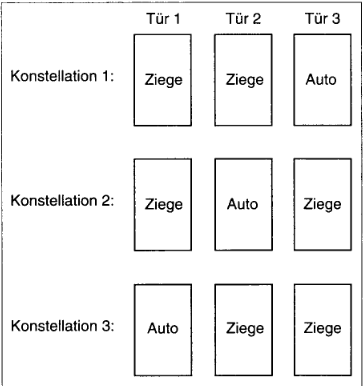
\includegraphics[scale=0.5]{erklaerung}
		}
	\frame{
		\frametitle{Verdeutlichung}
		Würdet ihr wechseln, wenn es 1000 Türen gäbe und 998 davon geöffnet werden?
		}
		\frametitle{Quellen}
		\url{https://de.wikipedia.org/wiki/Hausziege#/media/Datei:Hausziege_04.jpg}\\
		\url{https://thumbs.dreamstime.com/b/drei-t\%C3\%BCren-1875644.jpg}\\
		\url{https://www.grin.com/document/214288}
\end{document}
